\chapter{Implementation}
\chlab{implementation}

Here will be implementation details about the three systems\ldots

\nlipsum


\begin{sidewaysfigure}[p]
\begin{center}
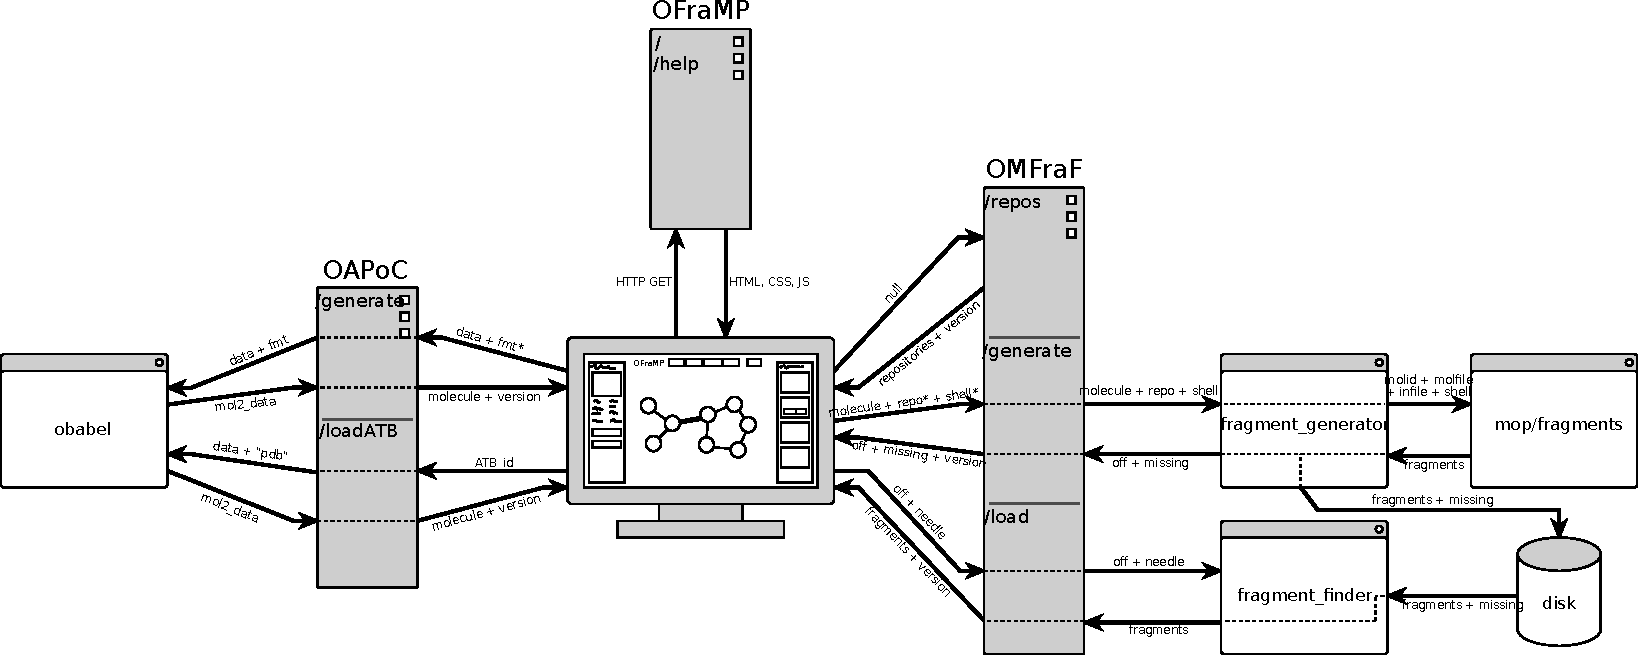
\includegraphics[width=\textwidth]{img/diagram.pdf}
\vspace{1em}
\caption{Schematic display of OFraMP and its supporting systems.}
\figlab{diagram}
\end{center}
\end{sidewaysfigure}


\section[OFraMP]{The Online tool for Fragment-based Molecule Parameterisation}
\nlipsum

\begin{figure}[h!]
\begin{center}
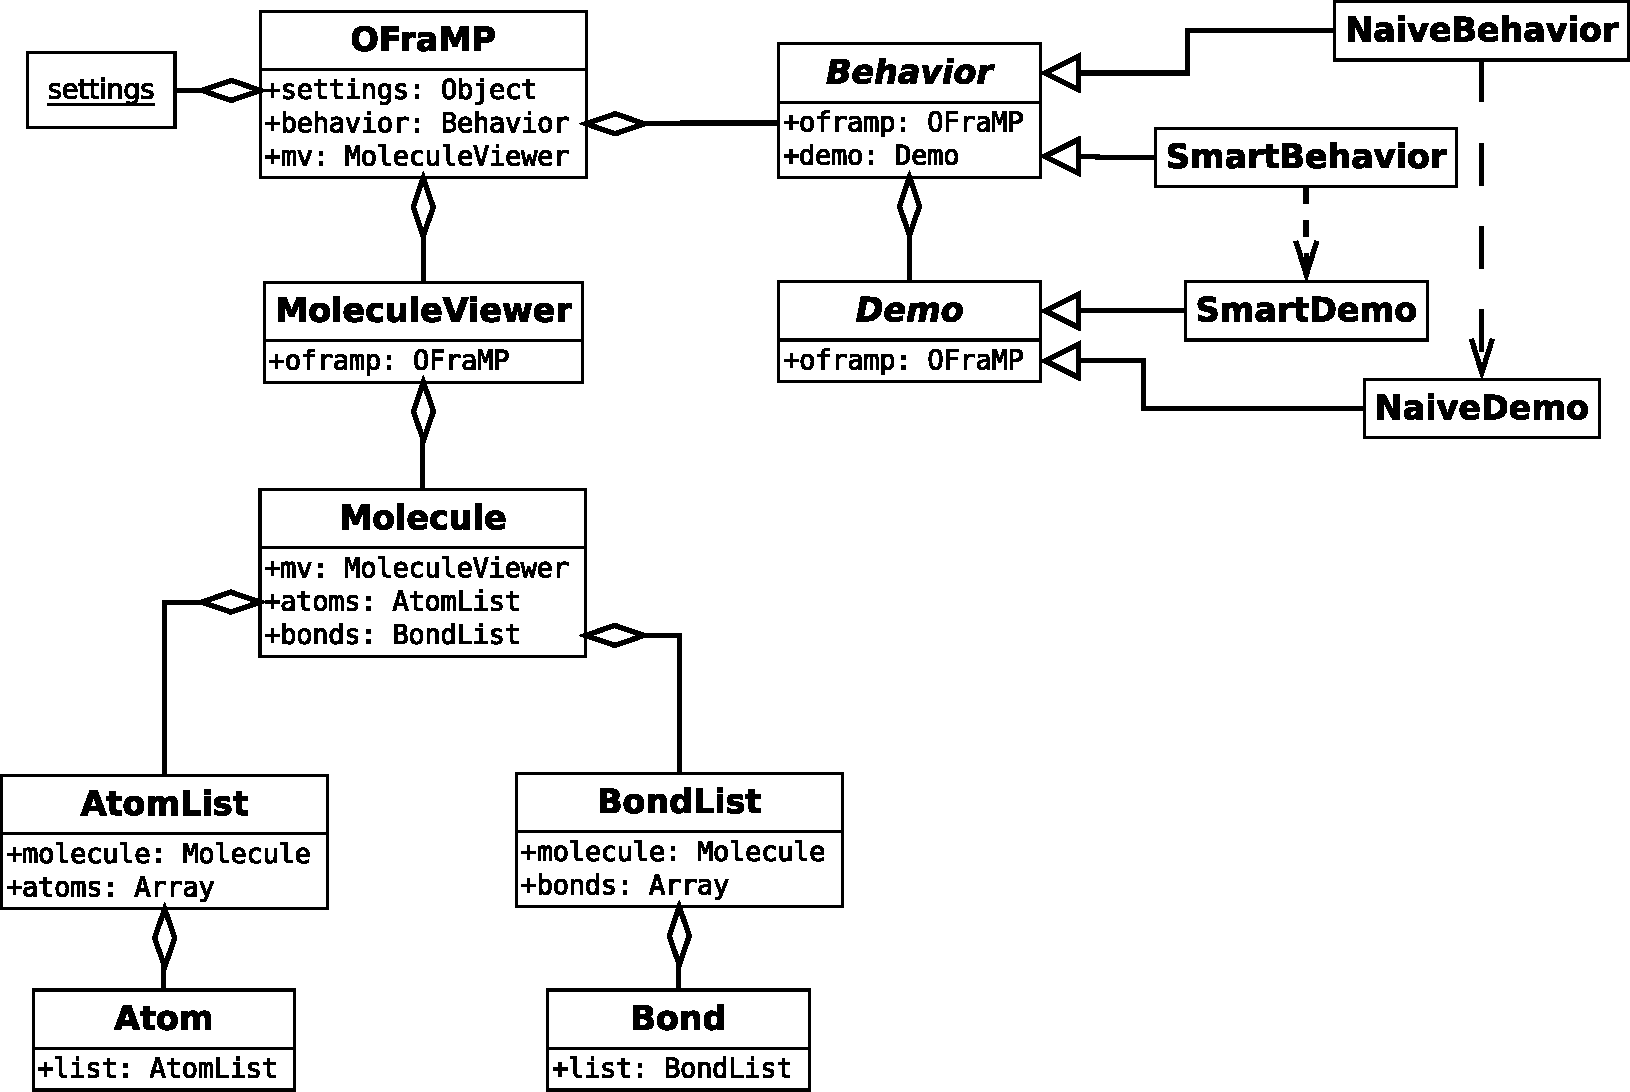
\includegraphics[width=\textwidth]{img/oframp_class.pdf}
\caption{Simplified class diagram of OFraMP}
\figlab{oframp_class}
\end{center}
\end{figure}

\subsection{Visualisation}
\nlipsum

\subsection{Interaction}
We use LGF files~\cite{dezso2011lemon}\ldots

\nlipsum


\section[OAPoC]{The Online tool for Atom Position Calculation}
\nlipsum

\subsection{obabel}
\nlipsum


\section[OMFraF]{The Online tool for Molecule Fragment Finding}
\nlipsum

\subsection{Generation}
\nlipsum

\subsubsection{mop/fragments}
\nlipsum

\subsection{Finding}
\nlipsum
